%
% aj - below -
%      We sometimes say view converges, sometimes view consistency
%      We should make sure these concepts are somewhat explained,
%      ideally, before we use them.

\section{View Maintenance System} 
\label{sec:view_maintenance_system} 

In this section, we present and discuss the design of \VMS. By
illustrating how a base table operation may effect a view table, we
provide the intuition for the resulting view consistency established
by \VMS.  Finally, we discuss fault-tolerance.

\subsection{Design Overview}

Figure~\ref{fig:view_maintenance_system} gives an overview of \VMS,
which is comprised of a \textit{coordinator} and an arbitrary number
of \textit{sub-systems}. The coordinator manages system load and
recovery, whereas the sub-systems -- more specifically the
\textit{view managers} (\VMs) in a sub-systems -- update views. The
input to \VMS\ is a set of operation streams ($ts_1$,$ts_2$..$ts_n$);
each emitted by a \KVS\ node (cf. Figure~\ref{fig:kv_model}).  Each
\VMS\ sub-system manages one stream of operations.  A sub-system
distributes the incoming operation stream to \VMs. The number of
\VMs\ per sub-system is configurable. \VMs\ can be dynamically
\textit{assigned} to or \textit{removed} from sub-systems. The
coordinator can also re-assign \VMs\ from one sub-system to another.

A \VM\ is designed to be light-weight and can be deployed in large
numbers to accommodate a changing view update load. It computes view
updates, based on base table operations it receives as input via the
\KVS\ API, for view tables. A \VM\ only belongs to a single
sub-system. The sub-system feeds the \VM\ with operations which
processes them in order.  A \VM\ is the unit of scalability of
\VMS. \VMs\ are kept stateless to be exchangeable at any time and to
minimize dependency. Given a number of view definitions and a sequence
of operations, a \VM\ is always able to execute any view table update
from any host.

\begin{figure}
  \centering
    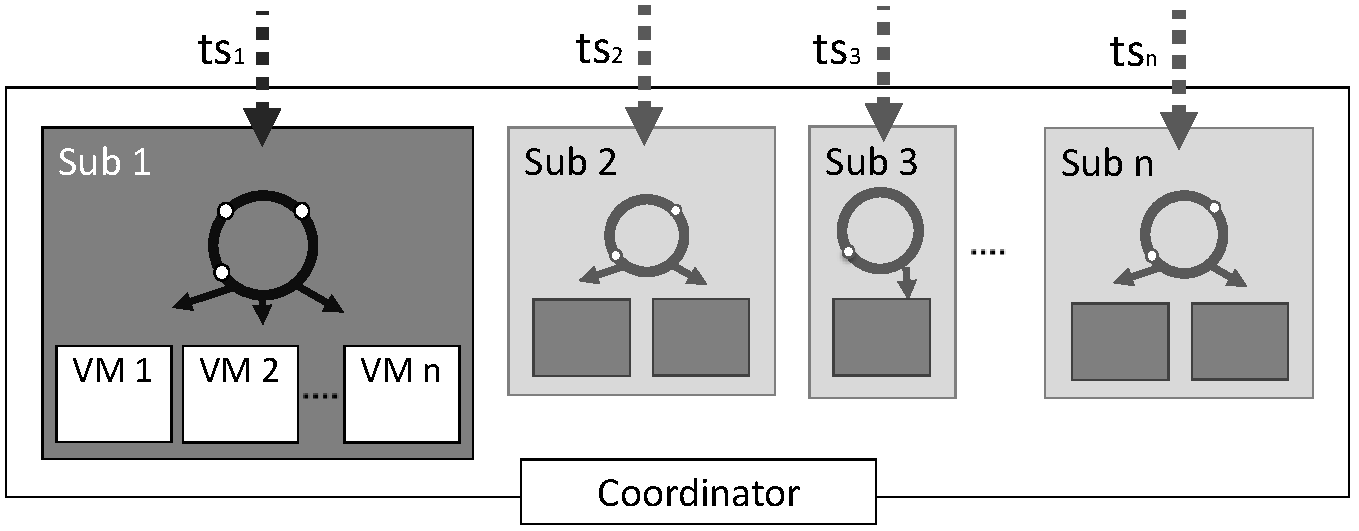
\includegraphics[width=\linewidth]{figures/ViewMaintenanceSystem}
    \caption{View Maintenance System (\VMS)}
    \label{fig:view_maintenance_system}
\end{figure}

Our design exhibits at least the following four benefits: (i) Seamless
scalability: Hundreds of views may have to be updated as a consequence
of a single base table operation. As \VMS\ exceeds its service levels,
additional \VMs\ can be spawned (below, we show this
experimentally). (ii) Operational flexibility: \VMs\ introduce
flexibility to the system architecture. All \VMs\ of a given
sub-system can be hosted together on the same node or each \VM\ can be
hosted at a different node. (iii) Accommodate load variations:
\VMs\ can be reassigned from one sub-system to another as base table
update load changes. (iv) Fault-tolerance: If a \VM\ crashes, another
\VM\ can take over and continue processing the operation stream.

\subsection{Update Propagation} 
\label{subsec:update_processing} 

A sub-system distributes the arriving base table update stream to its
\VMs\ via consistent hashing by maintaining a hash-ring
(cf. Figure~\ref{fig:review_consistency}), where active \VMs\ are
registered.  Row keys of arriving updates are hashed into the ring and
associated in clock-wise direction with active \VMs.  In this way, a
sub-system distributes operations uniformly across the available
\VMs\ and ensures that base table operations on the same row key are
always handled by the same \VM. On the one hand, this mechanism
ensures maximal degree of concurrency for update propagation, while
simultaneously guaranteeing the ordered propagation of base table
updates to view tables, setting the basis for view table consistency.

After a \VM\ has been selected (via the hash-ring) to process a
certain client operation, the sub-system inserts the operation into
its queue.  One queue for every active \VM\ exists to buffer the
incoming client operations.  A sending thread (which can be
deactivated on demand) fetches the operations one after the other and
sends them to the \VM.

Every \VM\ maintains its own transaction log, referred to as
\textit{\VM-log}. When receiving an operation, a \VM\ directly writes
it to the \VM-log. Just like the transaction log, the \VM-log is kept
available by the underlying file system, employing recovery mechanisms
in face of \VM\ crashes (e.g., in the case of \HB, the file system
redundantly replicates file blocks via HDFS.)

To access and update view tables, a \VM\ acts as a client to the \KVS,
using its standard client API. Given a base table operation (e.g., a
put on a base table $A$), the \VM\ retrieves and caches the view
definitions of the derived views (e.g., a \texttt{SELECTION} and
\texttt{COUNT} view $S$ and $C$, both derived from $A$). Then,
\VM\ runs the update program, and submits view table updates (to $S$
and $C$) via the client API. For some of the view types maintained,
the \VM\ has to query the view table first, as part of the update
logic; in a \texttt{COUNT} view, the \VM\ reads the current count from
the view before applying the delta of the base table operation. These
view queries are always get operations (i.e., single row accesses) and
can be evaluated quickly.


%To access and update a view table, a \VM\ acts as a client to the
%\KVS, using its standard client API. Given a base table operation, the
%\VM\ retrieves (and caches) the view definitions of the views derived
%from that particular base table. Then, the \VM\ runs the update
%program and submits view table updates via the client API. Depending
%on the view type maintained, the \VM\ first queries the view table as
%part of the update logic. For example, in a \texttt{SUM} view, the
%\VM\ reads the current sum from the view before applying the delta of
%the base table operation.  These view queries are always get
%operations (i.e., single row accesses) and are evaluated efficiently
%by the underlying store.

To allow for parallel updates of multiple \VMs\ on the same view
record, we use a test-and-set mechanism (as suggested in
\cite{jacobsen:viewmaintenance}).~\footnote{In \HB\ a
  \texttt{checkAndPut} method is provided to realize this
  mechanism. Most \KVSs\ offer a similar abstraction.} When updating a
table record, a \VM\ sees (tests) whether a record has been
concurrently modified between a read and an update.

\textit{Example:} Let two \VMs, $VM_1$ and $VM_2$ retrieve the value
of the same view record $(x1, \{(col, a)\})$. Let $VM_1$ add the delta
$b$ such that $(x1,\{(col,a+b)\})$ and $VM_2$ add the delta $c$ such
that $(x1,\{(col,a+c)\})$. Now let both \VMs\ write back their values
to the view. As a result one of the delta values (either $b$ or $c$)
is overwritten and is not reflected in the view. Using a test-and-set
method prevents the scenario. Assuming $VM_2$ writes second; when
trying to put the new value, the test-and-set method tests the old
value $a$.  It fails because the old record value changed concurrently
to $a+b$. Thus, $VM_2$ fetches the updated value and re-computes
$(x1,\{(col,a+b+c)\})$. This time, test-and-set succeeds and the
record is written.

%
% aj - I will have to come back to the below paragraph, time-permititng
%
% aj - below -
%      What if a VM crashes after the operation has been written to the VM log
%        and before the view has been updated (state persisted in ZK?)
%      Also, doing the below after every view table update, sounds a bit
%       heavy weight; is this really done?
%      Also, this may not be the place to discuss FT.
%
% ja - the state (of the current committed transaction) has to be persisted
%     in ZK. This definitly draws off some performance, but reliability
%     always comes with a cost. Acutally, i think it's not too bad since 
%     ZK is distributed. Likewise, writing the VM log to HDFS was not a big
%     factor during evaluation.  
%
%	  The only alternative is replaying the log from the region server. 
%	  Still we need to keep track of the current committed transaction in ZK.
%     This is what we favored in the beginning, but it is only convinient
%     with a small number of VMs per region server. Moreover, it
%     causes re-propagation of updates that had been already applied. It
%     changes the read-state of the TL. This is --and i can just speak
%     from intuition here-- error-prone. What has been read from TL and
%	  and transferred to a VM should remain there. Recovery should just
%	  affect the crashed VM and not the rest of the system.
%
%	  In general, this discussion is too detailed to start it here(it may be
%	  also too detailed for FT). I am a little bit clueless how to proceed.
%
%After a view table update, the \VM\ persists the current state of work
%-- that is, the \textit{sequence number} of the last processed client
%operation and the updated view table name. This state is kept in
%ZooKeeper. The coordinator can restore the state in case of a
%\VM\ crash. A new \VM\ can resume the work from this point onward.

\begin{figure}
  \centering
    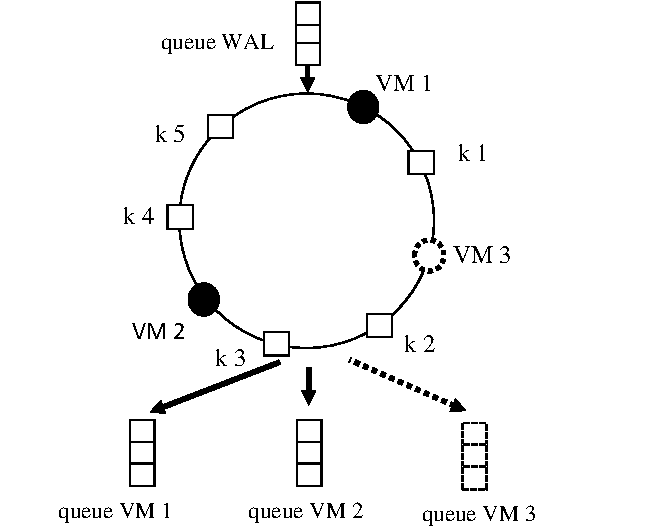
\includegraphics[width=\linewidth]{figures/ReviewConsistency}
    \caption{Sub-system setup}
    \label{fig:review_consistency}
    \vspace{-2mm}
\end{figure}



\subsection{Consistency Considerations} 

%
% aj - below - here is probably where we should describe what
%              consistency of views is and what convergence
%              means

%
%      We should discuss consistency here for what you call static
%      context and then later dynamic context.
% ja - in progress
%
% aj - in S4, we also say views are correct, smth. we should define
%      as well
% ja - i added a paragraph at the beginning of "consistency considerations"
%
%al.\cite{jacobsen:viewmaintenance} suggest,

Unconstrained incremental view maintenance and parallel propagation of
base table updates to views may result in the materialization of
inconsistent view data. By constraining how updates propagate,
\VMS\ prevents inconsistencies.

Informally speaking and considering that a base table constitutes a
\textit{sequence of base states} (one each resulting from the sequence
of client updates) and a view table a corresponding \textit{sequence
  of view states}. Then, view consistency can be defined via comparing
these two sequences.  Thus, a view is said to \textit{converge}, if a
correct final view state is reached (i.e., a view state that is
identical to evaluating the view expression over the final base table
state). A view is said to be \textit{consistent} if all intermediate
view states are \textit{correct} and \textit{ordered} according to the
base state sequence. That is, there are no view states that could
ever be derived from any base state (correctness). And, there is a
direct correspondence between both state sequences (i.e., racing base
updates will not lead to re-ordered view states)
(order).~\footnote{This description is intentionally kept
  informal. For a detailed formal analysis, see the technical
  reports~\cite{jacobsen:viewmaintenance, extendedpaper}.}
  
Based on the formal considerations in~\cite{jacobsen:viewmaintenance,
  extendedpaper}, we can proof that \VMS, which preserves timeline
of updates, applies view updates exactly once, and avoids ``backward
queries'' (to a base table), achieves
\textit{consistency}\footnote{What we refer to as \textit{consistency}
  here, is defined as \textit{strong consistency}
  in~\cite{jacobsen:viewmaintenance, extendedpaper}, which provides a
  more fine-grained shading of view table consistency.}.  Thus,
\VMS\ guarantees views converge and are consistent. Essentially, this
is the result of the mechanisms introduced above: consistent hashing
ensures that record timelines are respected in update propagation,
test-and-set and recovery mechanisms guarantee that view updates are
applied exactly once, finally, \VMS\ was designed to completely
dispense with backward queries
(cf. Section~\ref{sec:view_maintenance}).

These guarantees hold under the assumption of a ``static''
\VMS\ configuration: A fixed number of nodes and \VMs.  However, given
a ``dynamic'' context, where \VMS\ assigns and withdraws \VMs\ or
allows \KVS\ to add and remove nodes or move key-ranges, results in
the interference with view consistency, which we address below.


\subsubsection{Management Actions and Consistency} 

We now refine the behaviour of \VMS\ to allow for dynamic state
changes in sub-systems.  For reasons of recovery, load balancing and
scaling, \VMS\ performs the following actions: \textit{add}, makes the
\VM\ resource available to the \VMS; \textit{remove}, takes away a
\VM\ resource; \textit{assign}, makes a \VM\ available to a sub-system
such that it can process the sub-system's client operations;
\textit{withdraw}, takes away a \VM\ from a sub-system (opposite of
assign); and \textit{re-assign}, re-locates a \VM\ from one sub-system
to another. Adding a \VM\ to \VMS\ (or removing it) does not affect
view maintenance. The re-assign action is a combination of withdraw
and assign. Now, we explain how assign and withdraw actions are
performed safely (i.e., without interfering with consistency).

%\begin{table}
%\rowcolors{2}{gray!10}{gray!30}
%\setlength{\belowrulesep}{0pt}
%\setlength{\aboverulesep}{0pt}
%\setlength\extrarowheight{2pt}
%\begin{center}
%\begin{tabular}{l l l}
%\toprule
%Component & action & method \\
%\midrule
%View Manager & add & \textit{addViewManager()}  \\
% & remove & \textit{removeViewManager()}    \\
% & assign & \textit{assignViewManager()}  \\
% & withdraw & \textit{withdrawViewManager()}    \\
% & re-assign & \textit{reassignViewManager()}    \\
%\bottomrule 
%\end{tabular}
%\caption{\VMS\ actions}
%\label{tab:vms_events}
%\end{center}
%\end{table}

%Recall, that the sub-system selects the 
%responsible \VM\ by applying the hash function. The operation is then 
%inserted into the corresponding queue. 


\noindent
\textbf{Assign VM:} Figure~\ref{fig:review_consistency} shows how a
sub-system does view maintenance. Assume a new \VM\ (in the figure
represented by $V_3$) is assigned to the sub-system. The logic,
performed on the sub-system during the command, can be described as a
sequence of primitive actions: (1) Method $createQueue(vm)$ creates a
queue for a new \VM. (2) The \VM\ is added to the hash-ring by method
$insertHash(vm)$.  (3) The method $activateQueue(vm)$ starts the
sending thread that keeps transferring the queue's operations to the
\VM.

When a \VM\ is assigned, it is inserted into the hash-ring of the 
sub-system. Unless the hash-ring is empty, the new \VM\ is assigned a key 
range that is, at the same time, removed from another \VM. This leads
to violation of consistency (even convergence in terms of the consistency
model), as the following example shows.


\begin{algorithm}
\caption{Safe assignment procedure at sub-system}
\label{alg:assignvm}
\begin{algorithmic}
\Procedure{$assignVm$}{$vm_a, VM_{sub}$}
\State{$createQueue(vm_a)$}
\State{$insertHash(vm_a)$}
\ForAll{$vm \in VM_{sub}$}
\State{$queue(vm, m_a)$}\Comment{queue markers}	
\EndFor
\ForAll{$vm \in VM_{sub}$}
\State{$receiveAck(vm)$}\Comment{wait for acks}		
\EndFor
\State{$activateQueue(vm_a)$}	
\EndProcedure
\end{algorithmic}
\end{algorithm}


\textit{Example}: In Figure~\ref{fig:review_consistency}, $VM_1$ and
$VM_2$ are already assigned to the sub-system. They are responsible
for a certain range on the hash-ring; queues are feeding them with
incoming client operations. Assume a client performing a put operation
$p_1(k_1, \{..\})$; the sub-system receives $p_1$, selects $VM_2$ as
responsible and inserts $p_1$ into the queue of $VM_2$.  Now assume, a
new \VM\ $VM_3$ is assigned to the sub-system and its hash is inserted
within the range of $VM_2$ such that it acquires the responsibility
for key $k_1$. In a next step, a client sends an operation $p_2(k_1,
\{..\})$ to the same key. Because responsibility has changed, the
operation is sent to $VM_3$. Considering that $VM_3$ has just been
added, it's queue is empty and, hence, processes updates very fast. It
is likely to happen that $VM_3$ processes $p_2$ before $VM_2$ can
process $p_1$. Because both operations refer to the same base record,
the timeline of the record is broken and convergence is violated.

To process the assign command safely, we use so called \textit{markers}. 
Markers are -- just like client operations -- enqueued to a \VM\ and 
become a part of the operation stream. When the \VM, while processing 
operations, notices a marker, it replies with an acknowledgement back to 
the sub-system. Thus, the marker reveals to the sub-system, whether the \VM\ 
has completed all operations that were sent before the marker. We change the 
assignment procedure by adding a marker-based acknowledgement mechanism 
(cf. Algorithm~\ref{alg:assignvm}). 

%The
%algorithm is executed synchronously and if another assignment
%procedure is called on the sub-system, it must wait, until the first
%operation has terminated.
The procedure $assignVm$ takes two parameters: $vm_a$, the \VM\ that 
should be assigned to the sub-system, and $VM_{sub}$, a set of \VMs\ 
that are already assigned to the sub-system. The algorithm creates a 
queue for $vm_a$ and inserts it into the hash-ring. Then, it queues a 
marker $m_a$ to all assigned \VMs\ ($VM_{sub}$). After the sub-system 
has received acknowledgements from all \VMs, it is guaranteed that no 
operation in the key range of the newly added \VM\ $vm_a$ is still 
pending. Referring back to the above example: The timeline of $k_1$ can 
not be changed any more. 

%Operation $t_2$ has to
%wait in the queue of $VM_3$ until $VM_2$ acknowledges the processing
%of $t_1$ because the queue of $VM_3$ is activated only after the
%marker has been acknowledged and this, in turn, implies that operation
%$t_1$ has been processed.
\noindent
\textbf{Withdraw VM:} The logic, performed on the sub-system side
during a withdraw can be described analogously to the assign command
by a sequence of primitives (opposite actions in reverse order): (1)
$deactivateQueue(vm)$ stops the sending thread that keeps transferring
the operations in the queue to the \VM. (2) The \VM\ is removed from
the hash-ring by $removeHash(vm)$. (3) $deleteQueue(vm)$ removes the
queue for the withdrawn \VM. The queue can only be deleted, if it is
empty and no operation is queued.

\begin{algorithm}
\caption{Safe withdraw procedure at sub-system}
\label{alg:withdrawvm}
\begin{algorithmic}
\Procedure{$withdrawVm$}{$vm_w, VM_{sub}$}
\ForAll{$vm \in VM_{sub} \wedge vm \neq vm_w$}	
\State{$deactivateQueue(vm)$}
\EndFor
\State{$removeHash(vm_w)$}
\State{$queue(vm_w, m_w)$}\Comment{queue marker}
%\ForAll{$vm \in VM_{sub}$}
\State{$receiveAck(vm_w)$}\Comment{wait for ack}		
%\EndFor
\State{$removeQueue(vm_w)$}
\ForAll{$vm \in VM$}
\State{$activateQueue(vm)$}
\EndFor
\EndProcedure
\end{algorithmic}
\end{algorithm}

    
Also, during a withdraw procedure, consistency may be violated. At the
moment where a \VM\ is withdrawn, i.e., removed from the hash-ring,
its queue might still contain operations. If another \VM\ that
acquires the key range is fast enough, it might processes operations
before the withdrawn \VM\ has finished. Again, the timeline of base
records is changed. In order to prevent inconsistencies, we designed
Algorithm~\ref{alg:withdrawvm} analogously to
Algorithm~\ref{alg:assignvm}. It takes two parameters: $vm_w$, the
\VM\ that should be withdrawn from the sub-system, and $VM_{sub}$, the
set of \VMs\ that is assigned to the sub-system.

First, the queues of the \VMs\ that possibly increase their key range
on the hash-ring (i.e., all other \VMs) are deactivated. Then, a
marker $m_w$ is queued at the \VM\ that is withdrawn. If the \VM\ has
acknowledged the marker, the sub-system knows, that all operations
have been processed. It removes the queue of the \VM\ and re-activates
the queues of all \VMs.

\subsubsection{Fault-tolerance} 

Failure detection and recovery play a critical role in \VMS.  In this
section, we analyse the behaviour of \VMS\ under \VM\ and node crashes
to ensure that after appropriate recovery measures, views still
converge.

\noindent
\textbf{\VM\ crash} -- A \VM\ maintains a queue with operations
dispatched to it. During a \VM\ crash, these operations are lost, which
may result in non-converging views. Our recovery measures described
here, ensure view convergence under \VM\ crash. A \VM\ crash triggers an
event via ZooKeeper, notifying the \VMS\ coordinator.

First, the coordinator sends a withdraw command to the concerned
sub-system. The sub-system withdraws the crashed \VM\ from the
hash-ring and stops dispatching operations to it. This way no updates,
that were in-fight, while the \VM\ crashed, are lost. Next, the
coordinator starts a new \VM\ instance. Upon start-up, it tells the
new \VM\ to replay the \VM-log of the crashed \VM. The new
\VM\ contacts ZooKeeper and retrieves the last processed sequence
number of the crashed
\VM\ (cf. Section~\ref{subsec:update_processing}).  The new
\VM\ accesses the \VM\ log of the crashed \VM\ and -- starting from
the sequence number -- replays all the entries.

\noindent
\textbf{Node crash} -- A node crash is handled by the recovery
mechanism of the \KVS. The \KVS\ moves all key ranges of the crashed
node to other nodes. In case, client operations exist that were just
residing in memstore (and had not been written to the table file), the
\KVS\ replays the\TL. During replay, all operations are inserted into
memstore and directly flushed to disk.

The \TL\ of a crashed node is still available (due to replication in
the underlying file system, HDFS, for example.) Thus, the sub-system
that is streaming the operations from the crashed node's
\TL\ continues reading to the end of file. Now, that the stream (of
the crashed node's \TL) runs dry, \VMS\ re-assigns all \VMs\ to a
different sub-system.

Based on the above reasoning, we conclude that \VMS\ is able to
prevent loss and duplication of operations during crashes.


